\section{Sem'aforos}
Un sem'aforo es una variable especial protegida que constituye el m'etodo cl'asico para restringir o permitir el acceso a recursos compartidos (por ejemplo, un recurso de almacenamiento del sistema o variables del código fuente) en un entorno de multiprogramac'ion. Fueron inventados por Edsger Dijkstra y se usaron por primera vez en el sistema operativo THEOS.
Con este simulador permitimos armar los sem'aforos de Dijkstra y simular su comportamiento al crear procesos que requieren el acceso a la zona cr'itica.
Veamos un ejemplo para clarificar su comportamiento y forma de uso.

\begin{figure}
\centering
 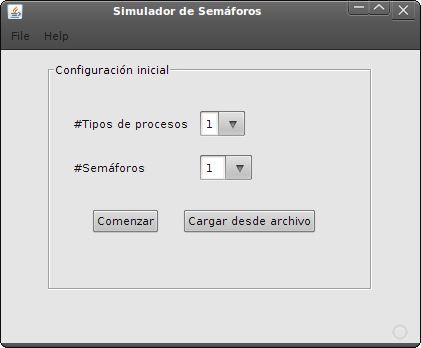
\includegraphics[scale=0.4,keepaspectratio=true]{./imagenes/semaforo/semaforos1.png}
 \caption{En la primer pantalla del simulador podemos elegir la cantidad de tipos de procesos y la cantidad de sem'aforos a utilizar, tambi'en podemos optar por cargar los datos desde un archivo.}
\end{figure}

\begin{figure}
\centering
 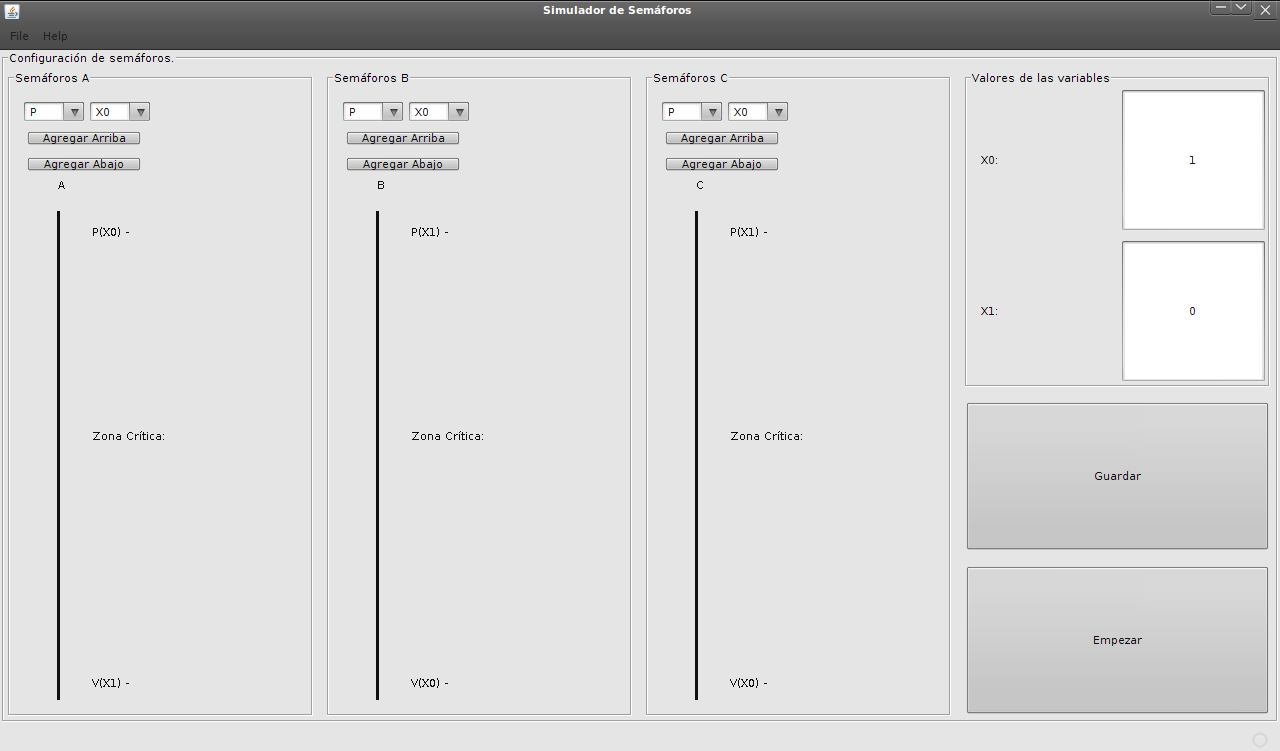
\includegraphics[scale=0.4,keepaspectratio=true]{./imagenes/semaforo/semaforos2.png}
 \caption{Ya en la segunda pantalla tenemos todas las herramientas para completar la configuraci'on de nuestro sem'aforo. Con los combos y los botones \emph{Agregar Arriba}, \emph{Agregar Abajo} y completando los valores de las variables podemos armar todos los sem'aforos que queramos modelar. En este ejemplo hemos completado con algunos operadores \emph{P} y \emph{V}, tambi'en seteamos los valores de \emph{X0} y \emph{X1}. Este ejemplo admite \emph{A(B}$|$\emph{C)}.}
\end{figure}

\begin{figure}
\centering
 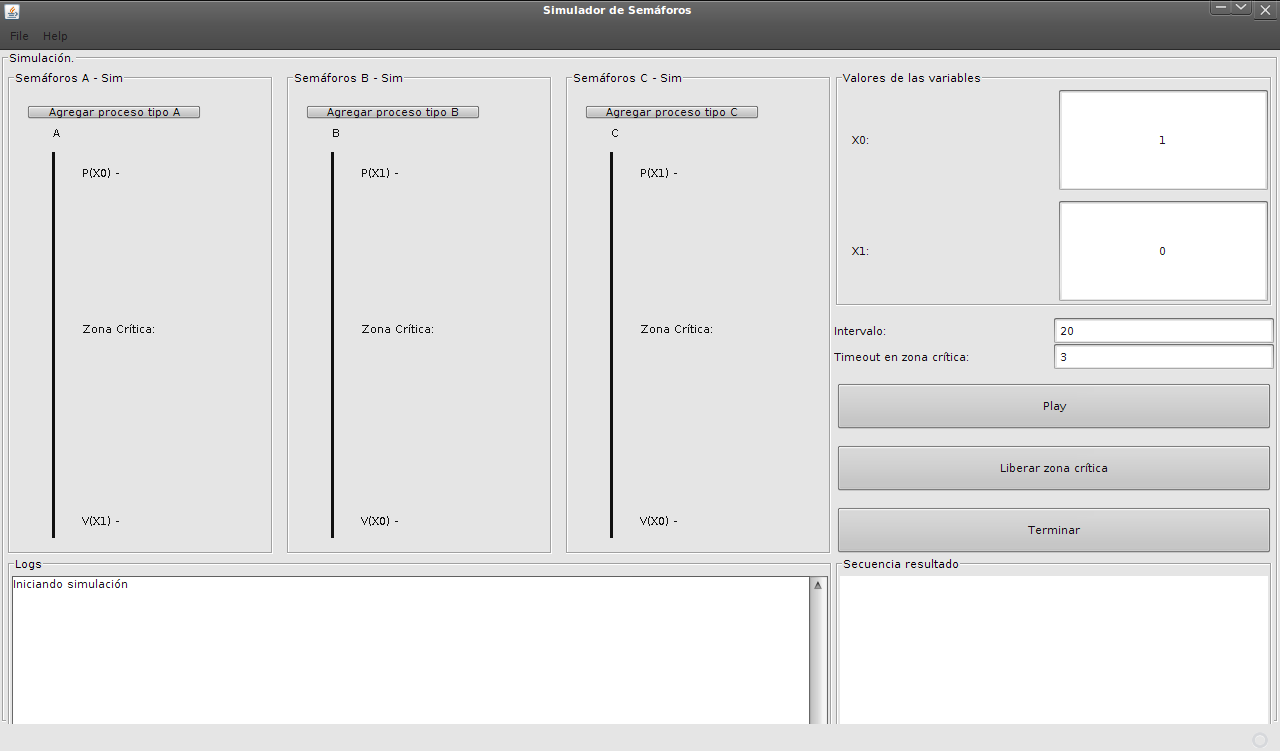
\includegraphics[scale=0.4,keepaspectratio=true]{./imagenes/semaforo/semaforos3.png}
 \caption{En la tercer pantalla podemos agregar procesos de cualquier tipo, setear los intervalos de tiempo correspondientes a la zona cr'itica y la velocidad del algoritmo en ejcutarse. El bot'on \emph{Liberar zona cr'itica} saca al proceso que est'e en la zona cr'itica en ese momento dando lugar al siguiente proceso. Podemos adem'as monitorear los valores de las variables de los sem'aforos, en el campo \emph{Secuencia resultado} podemos ver los tipos de procesos que han utililzado la zona cr'itica y en el campo \emph{Logs} podemos ver todo lo que ya ocurri'o en cada ejecuci'on.}
\end{figure}

\begin{figure}
\centering
 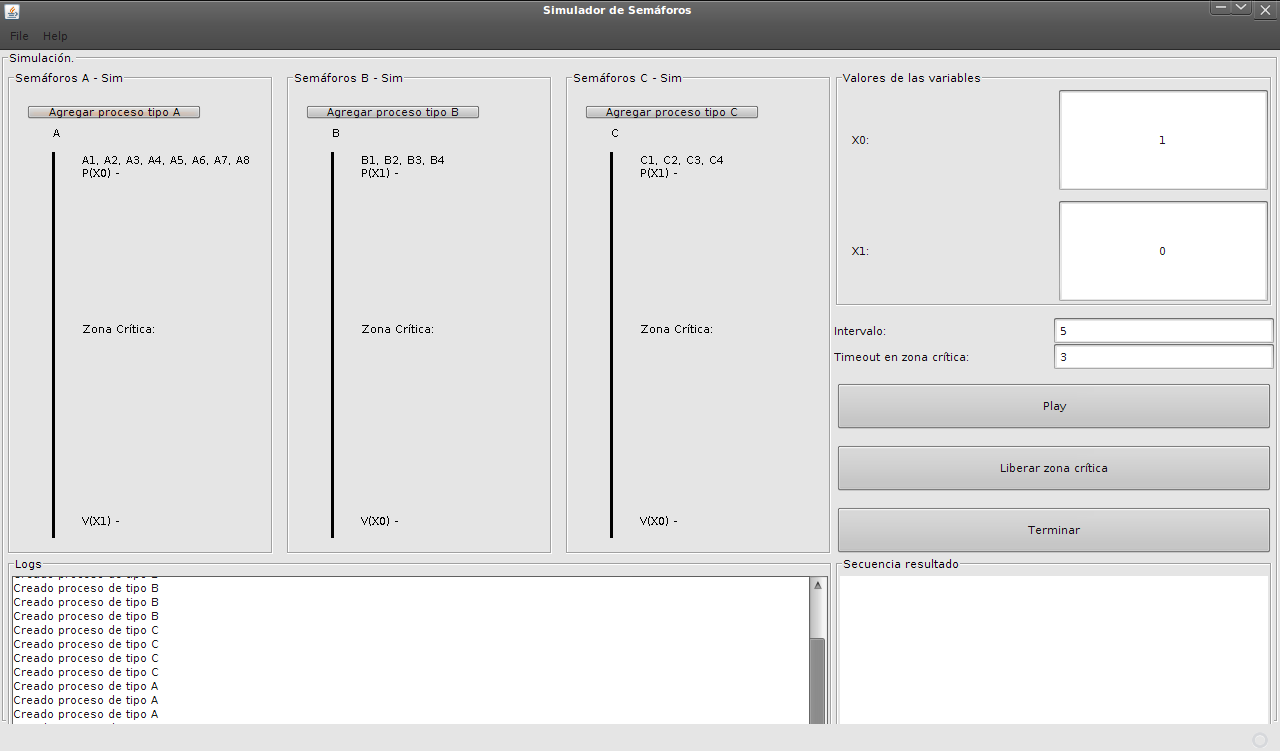
\includegraphics[scale=0.4,keepaspectratio=true]{./imagenes/semaforo/semaforos5.png}
 \caption{Agregamos distintos procesos de todos lo tipos para mostrar la ejecuci'on del simulador.}
\end{figure}

\begin{figure}
\centering
 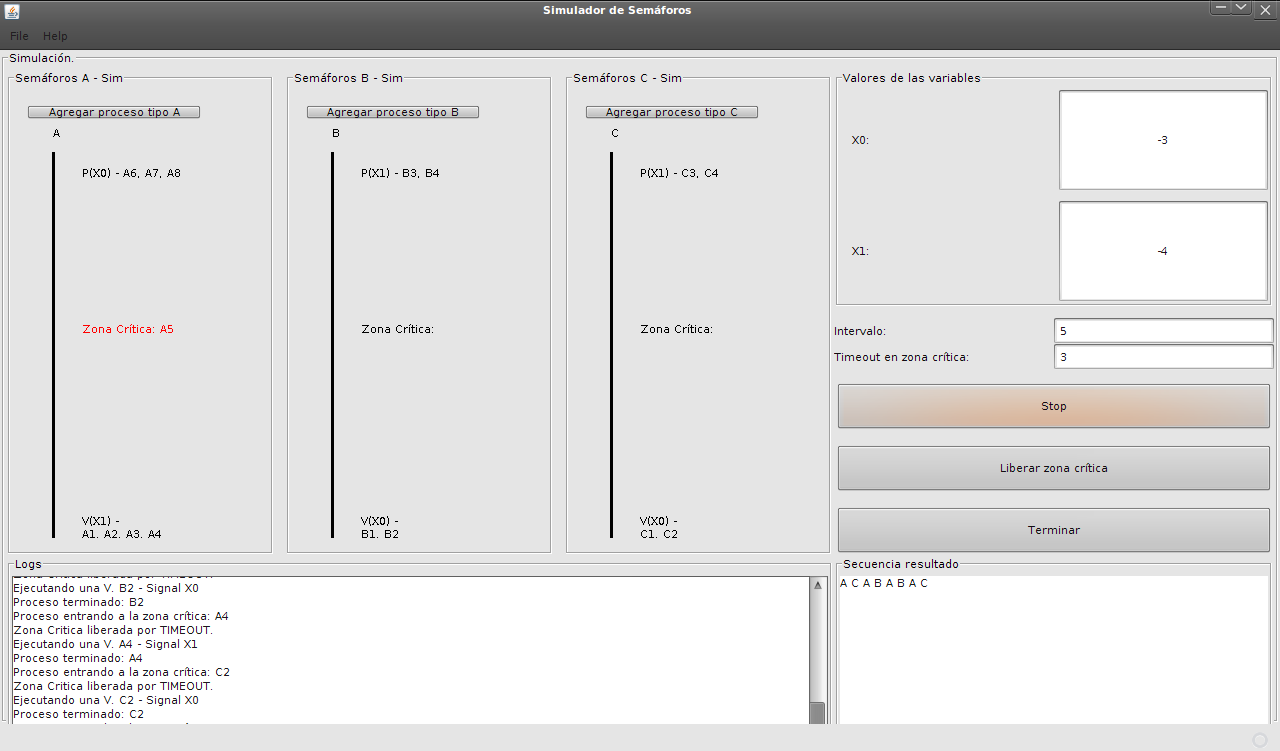
\includegraphics[scale=0.4,keepaspectratio=true]{./imagenes/semaforo/semaforos6.png}
 \caption{Por 'ultimo, el simulador en acci'on. En este momento podemos notar al proceso \emph{A5} ocupando la zona cr'itica. La \emph{Secuencia Resultado} concuedra con lo esperado.}
\end{figure}